\documentclass[a4paper,11pt,DIV=12,overfullrule=on]{scrreprt}%
\usepackage{unicode-math}%
\usepackage{polyglossia}%
\setdefaultlanguage{german}%
\setotherlanguage{english}%
\setmainfont[Mapping=tex-text]{Raleway}%
\setmonofont[Mapping=tex-text, Scale=0.9]{Fira Code Light}%
\setmathfont{Asana Math}%

\usepackage{xltxtra}%
\usepackage{microtype}%
\usepackage[svgnames, x11names, xetex, rgb, RGB, HTML, hyperref]{xcolor}%
\definecolor{shortyblue}{HTML}{1976D2}  % FIXME: Echte Farbwerte eintragen
\usepackage{listings}
\lstset{basicstyle=\ttfamily, numbers=left}
\definecolor{background}{HTML}{EEEEEE}
\definecolor{eclipseStrings}{RGB}{42,0.0,255}
\definecolor{eclipseKeywords}{RGB}{127,0,85}
\colorlet{numb}{magenta!60!black}

\lstdefinelanguage{json}{
    basicstyle=\normalfont\ttfamily,
    commentstyle=\color{eclipseStrings}, % style of comment
    stringstyle=\color{eclipseKeywords}, % style of strings
    numbers=left,
    numberstyle=\scriptsize,
    stepnumber=1,
    numbersep=8pt,
    showstringspaces=false,
    breaklines=true,
    frame=lines,
    backgroundcolor=\color{background}, %only if you like
    string=[s]{"}{"},
    comment=[l]{:\ "},
    morecomment=[l]{:"},
    literate=
        *{0}{{{\color{numb}0}}}{1}
        {1}{{{\color{numb}1}}}{1}
        {2}{{{\color{numb}2}}}{1}
        {3}{{{\color{numb}3}}}{1}
        {4}{{{\color{numb}4}}}{1}
        {5}{{{\color{numb}5}}}{1}
        {6}{{{\color{numb}6}}}{1}
        {7}{{{\color{numb}7}}}{1}
        {8}{{{\color{numb}8}}}{1}
        {9}{{{\color{numb}9}}}{1}
}

\usepackage[xetex, hyperindex, pdfpagelabels]{hyperref}
\hypersetup{
pdfauthor = {Markus Rennings},
pdftitle = {Shorty – URL-Shortener, Gruppe 3, Projektphase 2},
pdfsubject = {Projektdokumentation Shorty},
pdfkeywords = {Projekt, Projektphase, aws2302, Shorty, URL-Shortener},
pdfcreator = {XeLaTeX with hyperref package},
pdfproducer = {pdfLaTeX},
colorlinks = true,
linkcolor = shortyblue,          % color of internal links
citecolor = green,        % color of links to bibliography
filecolor = magenta,      % color of file links
urlcolor = shortyblue,          % color of external links
breaklinks = true,
}
\usepackage{graphicx}
\graphicspath{ {img/} }%
\usepackage{acronym}%


% Title Page
\subject{Projekt 2, Gruppe 3}
\title{Shorty – URL-Shortener}
\subtitle{}
\author{Andreas Brühl\thanks{Datenbank} \and Deniz Durmaz\thanks{Design, Frontend, Doku} \and Sebastian Hufeld\thanks{Design, Datenbank} \and Jason Krimmel\thanks{Design, Frontend} \and Markus Rennings\thanks{API-Design, Backend, OpenAPI, Doku, \XeLaTeX}}
\date{23.\,August–5.\,September~2023}
\publishers{Betreut durch: Martin Dubb, Fabio Keller}


\begin{document}
\raggedbottom%
\maketitle

\tableofcontents

% ! 1. Einleitung
\chapter{Einleitung}
\section{Kontext der Arbeit}
Das Projekt wurde im Rahmen einer geförderten Weiterbildung erstellt. Der Träger der Weiterbildung ist die Techstarter GmbH\footnote{\href{https://techstarter.de/}{https://techstarter.de/}}. Es gab mehrere Projekte zur Auswahl mit freier Gruppen- und Themenfindung. Das gewählte Projekt ist ein URL Shortener.

\section{Motivation für diese Arbeit}
In der Weiterbildung wurden verschiedene Methoden und Themenbereiche vermittelt. Diese sollen und werden in diesem Full-Stack-Projekt zusammengeführt und genutzt. So soll zum einen gezeigt werden, wie wir diese vielen Teilbereiche nutzen, um das Projekt umzusetzen.

Die größte Problematik ist es, sich erst einmal als Gruppe zu finden, aufzuteilen und zu sortieren, um die Anforderungen umzusetzen.

\section{Zielstellung für diese Arbeit}
Unsere Lösung wandelt lange \ac{URL} in kurze und eindeutige \ac{URL}s um. Bei \ac{URL}s kann die Zeichenlänge je nach Darstellung in mehreren Zeilen ausarten. Das kann zu Problemen in Dokumenten, E-Mails oder Social-Media-Posts führen. Durch die gekürzten \ac{URL}s wird dieses Problem behoben oder aber auch, wenn eine Zeichenbegrenzung vorhanden ist, wird diese nicht durch die lange \ac{URL} kannibalisiert. Optisch sind Short-\ac{URL}s ebenfalls nicht so aufdringlich.

\section{Anforderungen für diese Arbeit}
\begin{description}
    \item[URL-Validierung] Es ist erforderlich, eine \ac{URL}-Validierung zu implementieren, um sicherzustellen, dass die eingegebenen \ac{URL}s gültig sind.
    \item[URL-Kürzung] Die Lösung muss in der Lage sein, lange \ac{URL}s in kurze \ac{URL}s umzuwandeln.
    \item[Generierung von Kurzlink-Codes] Die Kurzlinks müssen eindeutig sein.
    \item[Benutzeroberfläche] Es muss eine benutzerfreundliche Oberfläche sein, über die Nutzer \ac{URL}s eingeben und Kurzlinks generieren können.
    \item[Anzeige von Kurzlinks] Benutzer bekommen bei Generierung des Kurz-Links ein Passwort mitgeteilt, mit dem sie sich die Statistik zu dem Link anschauen können. Diese Statistik umfasst eine Auswertung, wie oft auf den Link zugegriffen wurde, mit welchen Browsers und mit welchem \ac{OS}. Auch der Zeitpunkt des letzten Zugriffs wird ausgewertet.
    \item[Datenbank] Die Anwendung muss die ursprünglichen \ac{URL}s und die zugehörigen Kurzlinks in einer Datenbank speichern und die Verknüpfung zwischen ihnen sicherstellen.
    \item[API] Ein \ac{API} muss entwickelt werden, um die Interaktion zwischen Frontend und Backend zu ermöglichen. Dies ermöglicht das Erstellen und das Abrufen von Kurzlinks. Das gleiche gilt für die dazugehörigen Statistiken.
    \item[Statistik und Analyse] Die Anwendung muss die Daten über die Nutzung der generierten Kurzlinks sammeln und speichern. Einschließlich Anzahl der Klicks, Zeitpunkt der Nutzung und Informationen zu \ac{OS} und Browser der Nutzer, müssen generiert werden.
    \item[(Passwortschutz für Link-Bearbeitung und Statistik)] Jeder generierte Kurzlink muss über ein eindeutiges Schlüssel/Passwort verfügen, mit dem Benutzer den Link bearbeiten und die Statistiken einsehen können.
\end{description}

% ! 2. Technische Grundlagen
\chapter{Technische Grundlagen}
Grundsätzlich sind weitläufige Kenntnisse aus der Webentwicklung erforderlich, um die Architektur und die Komponenten des Full-Stack-Projekt umzusetzen und zu verstehen.

\begin{description}
    \item[Frontend- und Backend-Technologien] Grundlegende Kenntnisse über die Technologien, die im Frontend und Backend verwendet werden, wie z.\,B. \ac{JS} oder react.js, um die Benutzeroberfläche und die Serverseite zu entwickeln und gestalten.

    \item[Datenbank] Verständnis von Datenbankkonzepten und -operationen, insbesondere der Speicherung und Abfrage von Daten.

    \item[API] Schnittstellen-Bildung und Integration zur Sicherstellung einer fehlerfreien Kommunikation zwischen den einzelnen Elementen.

    \item[Sicherheit] Sichere Speicherung von gestellten Anfragen, Benutzern und Passwörtern.

    \item[Statistik und Daten] Speicherung, Abruf und Visualisierung der vorhanden bzw.\ angefragten Daten (\ac{URL}, Klicks) für die Erstellung der Statistik.
\end{description}

\section{Benutzeroberfläche}
\section{Datenbank}
\subsection{Datenbank-Struktur}
\section{Statistik und Analyse}
Für die Statistik nutzen wir die Express.js-Middleware {\ttfamily express-useragent}\footnote{\href{https://www.npmjs.com/package/express-useragent}{https://www.npmjs.com/package/express-useragent}}, welches die User-Agent-Kennungen zusammenfasst, so dass man nicht für jede Browser-Version einzeln checken muss. Diese Daten werden in der Datenbank kumuliert und bei Anfrage entsprechend über den \ac{API}-Endpunkt {\ttfamily /api/stats/\{shortUrl\}} an den Client gesendet. Die Statistiken sind mit einem Passwort geschützt, dass dem Benutzer bei Erstellung der Kurz-URL angezeigt wird.

\section{API}
Die \ac{API} bietet verschiedene Endpunkte für den Zugriff. So wird zur Erstellung eines Kurz-Links der http-POST-Endpunkt »{\ttfamily /}« genutzt, zur Weiterleitung (Abfrage des Kurz-Links) wird der GET-Endpunkt »{\ttfamily /\{shorturl\}}« verwendet. Und zur Abfrage der Statistiken dient der POST-Endpunkt »{\ttfamily /api/stats/\{shortUrl\}}«. 
\section{URL-Validierung}
Zur Validierung der URL nutzen wir das Paket {\ttfamily url-http}\footnote{\href{https://www.npmjs.com/package/url-http}{https://www.npmjs.com/package/url-http}} mit einer kleinen Wrapper-Funktion (siehe Abb.~\ref{fig:25wrapper}), wobei die \ac{URL} inklusive Schema ({\ttfamily http://} bzw. {\ttfamily https://}) erwartet wird.
\begin{figure}[h]%
    \begin{small}%
        \begin{center}%
            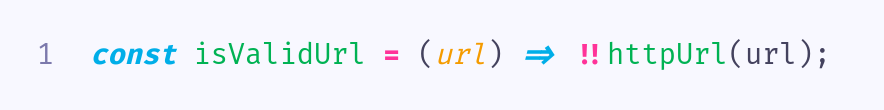
\includegraphics[width=0.8\textwidth]{2_5_wrapper.png}%
        \end{center}%
        \caption{Quelltextauschnitt der Wrapper-Funktion zur \ac{URL}-Validierung}%
        \label{fig:25wrapper}%
    \end{small}%
\end{figure}%

\section{URL-Kürzung}
Die eigentliche URL-Kürzung entsteht durch einen Datenbank-Eintrag, der die generierte Kurz-\ac{URL} (ID) mit der langen \ac{URL} verknüpft und zusätzlich die statistischen Daten zu jedem Kurzlink speichert.
\subsection{Algorithmus}
Wir haben uns für die Verwendung eines 58-stelligen Alphabets (Base-58) für die Generierung der ID entschieden. Hierzu werden von einem Base62-Alphabet ({\ttfamily[0–9A–Za–z]}) die Zeichen »0« (Null), »I« (Großbuchstabe i), »O« (Großbuchstabe o) und »l« (Kleinbuchstabe L) entfernt, da diese – je nach Schriftart – verwechselt werden können. Hierdurch wird zwar die Anzahl der möglichen IDs eingeschränkt, aber $58^7 =  2\,207\,984\,167\,552$ Möglichkeiten sollten diese immer noch ausreichen.

Die eigentliche Kurz-\ac{URL} ist dann ein siebenstelliger base58-kodierter String aus einer Kombination aus Teilen des Unix-Zeitstempels (Abb.~\ref{fig:261shorturl} Zeilen 1–3) und einer zweistelligen Zufallszahl (Zeile 4). Zum einfacheren Verbinden beider Zahlen werden diese zunächst als String generiert und erst bei Übergabe an die Funktion {\ttfamily base58()} als Integer umgewandelt (ebenfalls Zeile 4 in Abb.~\ref{fig:261shorturl}).
\begin{figure}[h]%
    \begin{small}%
        \begin{center}%
            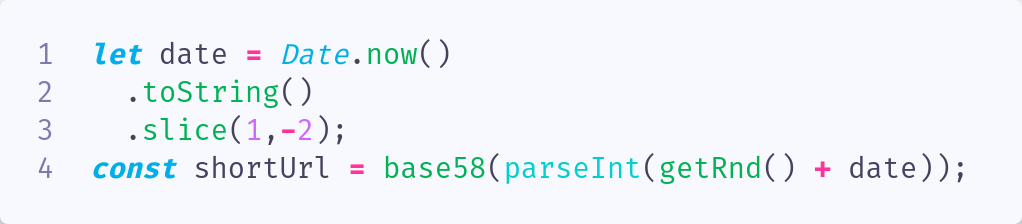
\includegraphics[width=0.8\textwidth]{2_6_1_shortUrl.png}%
        \end{center}%
        \caption{Quelltextauschnitt zur Generierung der Kurz-Url}%
        \label{fig:261shorturl}%
    \end{small}%
\end{figure}%


\section{Passwort für Link-Bearbeitung und Statistik}
Das Passwort für die generierte Kurz-\ac{URL} lassen wir uns als zufällige, zwölfstellige alphanumerische Zeichenkette durch das Modul »generate-password«\footnote{\href{https://www.npmjs.com/package/generate-password}{https://www.npmjs.com/package/generate-password}} erstellen.


% ! 3. Beschreibung der Lösung
\chapter{Beschreibung der Lösung}
\section{Software-Architektur der Lösung}
\section{Übersicht und Zusammenspiel der Komponenten}
\section{Beschreibung der Komponenten}
\subsection{Backend}
\subsubsection{Aufgaben der Komponente}
\subsubsection{Schnittstellen der Komponente}
Es gibt drei Schnittstellen der \ac{API}:
\begin{description}
    \item[/] POST-Endpunkt, um eine neue Kurz-\ac{URL} zu generieren
    \item[/\{shortUrl\}] GET-Endpunkt, um eine Kurz-\ac{URL} abzurufen. Der Abrufende wird automatisch, mittels http-Status 302, an die Zieladresse weitergeleitet.
    \item[/api/stats/\{shortUrl\}] POST-Endpunkt zum Abruf der Statistik zu der angegebenen Kurz-\ac{URL}. Das Passwort muss im Request-Body gesendet werden.
\end{description}
Für eine genaue (technische) Dokumentation haben wir die \ac{API}-Dokumentation im OpenAPI-Format erstellt, welche über das Backend\footnote{\href{http://localhost:8080/api/doc/api}{Backend:Port/api/doc/api}} abrufbar ist.
\subsubsection{Datenstrukturen}
Die Daten werden in einer Document-Database (Google Firebase Firestorm\footnote{\href{https://firebase.google.com/}{https://firebase.google.com/}}) gespeichert, und können im \ac{JSON}-Format abgerufen und geschrieben werden.

Wir haben uns für eine recht einfache Struktur entschieden:
\begin{lstlisting}[language=json]
{
    "clicks": 0,
    "lastClick": timestamp,
    "OS": {
        "Linux": 0,
        "Windows": 0,
        "MacOs": 0,
    },
    "Browser": {
        "Chrome": 0,
        "Edge": 0,
        "Firefox": 0,
        "Opera": 0,
        "Safari": 0,
        "Sonstige": 0,
    },
    "createDate": timestamp,
    "expireDate": timestamp,
    "longURL": "http://ex.amp.le/",
    "shortURL": "aB1Cd2e",
    "Password": "password"
}
\end{lstlisting}
\subsubsection{Funktionsweise}
\subsection{Frontend}
\subsubsection{Sub-Komponente 1}
\paragraph{Aufgabe der Komponente}
\paragraph{Schnittstellen der Komponente}
\subsubsection{Sub-Komponente 2}
\section{Übersicht Verzeichnisse und Dateien}
\section{Bauen des Gesamtsystems}
Ist dies nicht Kapitel 4.1?


% ! 4. Einrichtung und Betrieb der Software-Lösung
\chapter{Einrichtung und Betrieb der Software-Lösung}
\section{Inbetriebnahme der Lösung}
\section{Möglichkeiten zur späteren Anpassung und Weiterentwicklung}
Es bestehen diverse Möglichkeiten, das Projekt weiterzuentwickeln:
\begin{itemize}
\item Die Statistiken können erweitert werden, so dass man auch nach mobilen (Smartphone, Tablet) oder stationären (Desktop/Laptop, Smart-TV) auswerten kann.
\item Auch können die \ac{API}-Endpunkte erweitert werden, so dass z.\,B. nur Werte zu einer bestimmten Statistik abgerufen werden können.
\item Es kann auch dahingehend erweitert werden, dass sich Benutzer registrieren und anmelden können. Dann kann auch für den eingeloggten Nutzer ein Verlauf der generierten Kurz-\ac{URL}s angezeigt werden und die jeweiligen Statistiken mit einem einfachen Button aufrufbar gemacht werden.
\item Es kann ein DELETE-Endpunkt implementiert werden, damit ein Benutzer seinen generierten Link vorzeitig löschen kann.
\item Die generierten Links sollten auch nach einer voreingestellten Zeit automatisch gelöscht werden. Diese Zeit kann bis zu einer Obergrenze von Nutzer festgelegt werden. Das Löschen selbst kann beispielsweise durch einen Endpunkt erfolgen, der von außen mitteln {\ttfamily cron} und {\ttfamily curl} angesprochen wird. Das Feld {\ttfamily expireDate} ist schon in jedem Datensatz enthalten und wird standardmäßig auf Erstellungszeit + 30 Tage gesetzt.
\end{itemize}

% ! 5. Retrospektive
\chapter{Retrospektive}
\section{Evaluierung der Projektergebnisse}
\section{Bewertung der eigenen Arbeitsweise und die Zusammenarbeit im Team}
\section{Gewonnene Erkenntnisse für zukünftige Projekte}

% ! 6. Zusammenfassung und Ausblick
\chapter{Zusammenfassung und Ausblick}

\chapter*{Liste der Abkürzungen}
\begin{acronym}
    \acro{API}{Application Programming Interface (Programmierschnittstelle)}
    \acro{JS}{Javascript}
    \acro{JSON}{Javascript Object Notation}
    \acro{OS}{Operating System (Betriebssystem)}
    \acro{URL}{Uniform Resource Locator}
\end{acronym}

%\listoftables
\listoffigures
\end{document}
